\documentclass{article}
% option ``report'' puts title on separate page

\usepackage{amsmath}
\usepackage[pdftex]{graphicx}

\begin{document}

\title{WS6: Linear Systems of Equations and Stiff ODEs}
\author{Jackie Villadsen}
\date{\today}
\maketitle


\section{Solving Large Linear Systems of Equations}

\begin{figure}[h]
  \begin{center}
     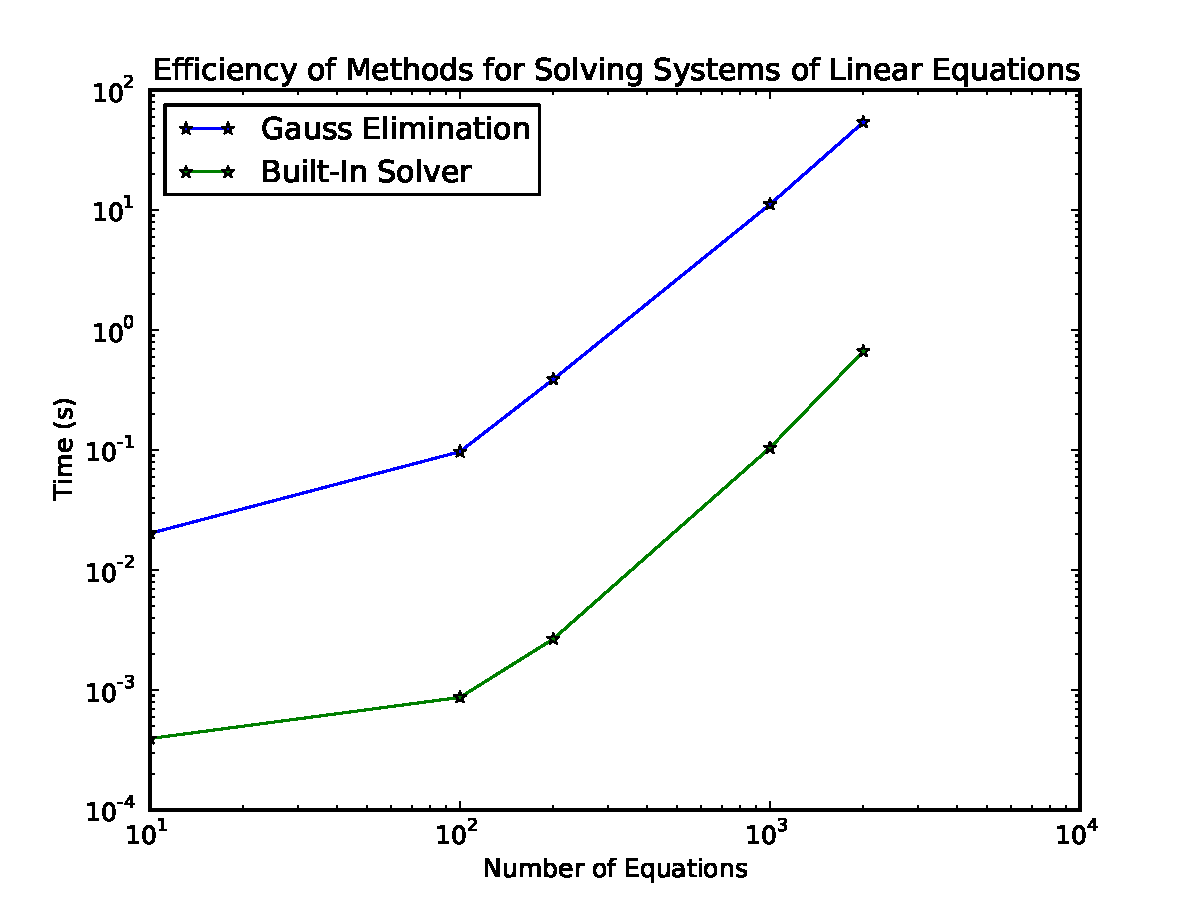
\includegraphics[width=\textwidth]{linsystimes}
  \end{center}
  \label{fig:times}
\end{figure}

I calculated the determinant of each of the professor's miraculous sets of
supernova-solving linear equations to check that they are solvable.  Table
\ref{tab:linsys} shows each system's size and determinant, as well as times to
solve the systems by two different methods.  All the systems have non-zero
determinants (the determinants of systems 4 and 5 are not actually infinite, but
are so large that python decided they were infinite), so all the systems are solvable.
I compared the efficiency of Gaussian elimination and back-substitution to that of
python's built-in solver for large systems of linear equations.  I found code
for Gaussian elimination and back-substitution online at
http://snippets.dzone.com/posts/show/5645, and compared it to the solve() function from
numpy.linalg.  The solve() function uses LU decomposition, which is of the same
order O($n^3$) as Gaussian elimination, but has a smaller proportionality constant.
Gaussian elimination and back-substitution is similar to how I would solve a linear
system of equations by hand - convert it to upper triangular form and then use back-substitution
to solve.  LU decomposition relies on factoring the matrix A into two matrices L and U (A=LU),
the first of which is lower triangular and the second of which is upper triangular, and then using
forward- or back-substitution to solve a system with each of those.
In Figure \ref{fig:times}, we see that the run times for Gaussian elimination and LU
decomposition have roughly the same slope on a log-log plot, so they are of the same order.

\begin{table}[p]
\centering
\begin{tabular}{|l|l|l|l|l|}
\hline
i & Number of Equations & Determinant & Gauss Elimination (s) & Built-In Solver (s) \\
\hline
1 & 10 & 0.0107 & 1.4e-3 & 1.5e-4 \\
2 & 100 & -3.08e33 & 9.4e-2 & 3.8e-4 \\
3 & 200 & -1.52e98 & 0.38 & 1.8e-3 \\
4 & 1000 & -inf & 11 & 1.2e-1 \\
5 & 2000 & inf & 54 & 0.68 \\
\hline
\end{tabular}
\label{tab:linsys}
\end{table}

\section{Stiff ODE Systems}
For the system of ODEs
\begin{subequations}
\begin{equation}
	\frac{dY_1}{dt} = Y_1 - 99 Y_2
\end{equation}
\begin{equation}
	\frac{dY_2}{dt} = - Y_1 + 99 Y_2
\end{equation}
\end{subequations}
the analytic solution is:
\begin{subequations}
\begin{equation}
	Y_1(t) = \frac{1}{100} e^{100t} + \frac{99}{100}
\end{equation}
\begin{equation}
	Y_2(t) = - \frac{1}{100} e^{100t} + \frac{1}{100}.
\end{equation}
\end{subequations}

\begin{figure}[h]
  \begin{center}
     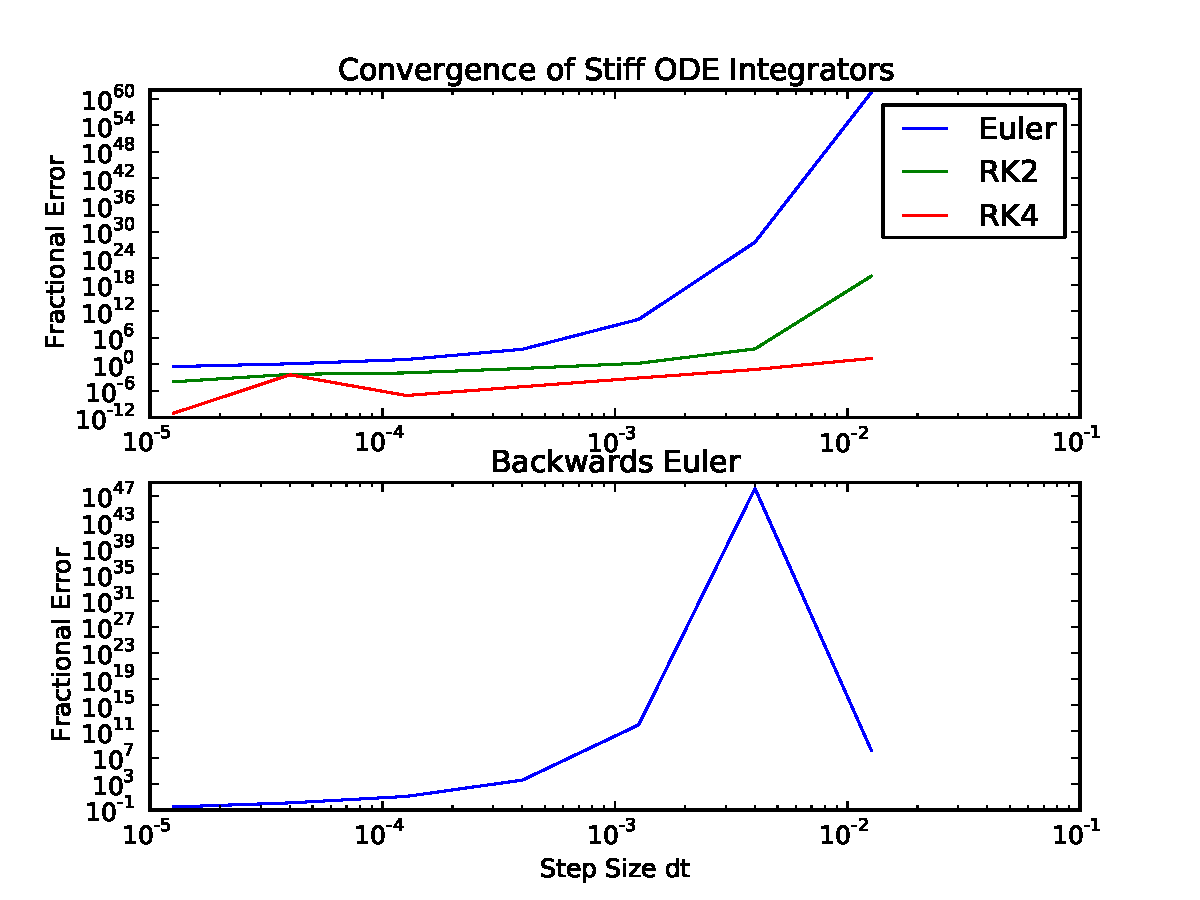
\includegraphics[width=\textwidth]{stiff}
  \end{center}
  \label{fig:stiff}
\end{figure}

I used a variety of different integration methods to integrate
from t=0 to t=4 for the initial conditions $Y_1(t=0)=1$ and
$Y_2(t=0)=0$.  For the different methods, and a range of step sizes,
I calculated a ``fractional error'' $(Y_{numeric}-Y_{analytic})/Y$, where $Y_{numeric}$ is
the numerically calculated value for Y(t=4), $Y_{analytic}$ is the
analytic value, and $Y$ is the larger of the two.  For too-large step sizes for forwards
Euler and Runge-Kutta of orders 2 and 4, the analytic value came out many orders of magnitude
larger than the numerical value.  For backwards Euler, the numerical value came out orders
of magnitude larger than the analytic value.  An interesting thing I noticed, when playing
with step sizes, is that even as the fractional error reached small percentages (less than
1\%), it would still vary erratically and widely as I systematically increased the step size.
Figure \ref{fig:stiff} shows how fractional error depends on step size for a few different
step sizes (I only picked a few in order to limit calculation time).  RK4 reached low fractional
error for the largest step size, followed by RK1, and backwards and forwards Euler were
comparable.


\end{document}